%Este trabalho está licenciado sob a Licença Creative Commons Atribuição-CompartilhaIgual 4.0 Internacional. Para ver uma cópia desta licença, visite https://creativecommons.org/licenses/by-sa/4.0/ ou envie uma carta para Creative Commons, PO Box 1866, Mountain View, CA 94042, USA.

\chapter{Teoria de conjuntos}

%Texto baseado em Topologia-Elon e \cite{munkres}.

Chamamos de \textbf{conjunto} uma coleção de objetos que satisfazem uma propriedade comum. Usaremos letras maiúsculas $A, B, \ldots$ para representar  conjuntos, e letras minúsculas $a, b, \ldots$ para representar seus elementos.

A notação $x \in A$ (lê-se ``$x$ pertence a $A$'') significa que $x$ é um elemento de $A$. A notação $x \notin A$ (lê-se ``$x$ não pertence a $A$'') significa que $x$ não é um elemento de $A$.

Dados os elementos $a, e, i, o, u$ indica-se com $\{a, e, i, o, u\}$ o conjunto que é formado por estes elementos. Assim, por exemplo, $V= \{a, e, i, o, u\}$ é o conjunto das vogais do alfabeto português, quando representamos um conjunto desta forma dizemos que estamos representando o conjunto por enumeração de seus elementos.

Assim se denotarmos por $U$ o conjunto formado pelas letras do alfabeto português, como toda vogal é uma letra do alfabeto português, podemos representar o conjunto $V$ da seguinte forma:
\begin{equation}
V= \{x \in U \mid x \text{ é uma vogal}\}
\end{equation}
aqui $x$ representa um elemento qualquer do conjunto $U$.

Esta segunda forma que usamos para descrever o conjunto $V$ é uma forma usual de descrever conjuntos na matemática, perceba que nela começamos pensando em um conjunto ``grande'' $U$ (que chamamos de conjunto universo) e em uma propriedade $P$ bem particular que alguns elementos deste conjunto satisfaziam, e assim obtemos o conjunto $V$.

Além de relacionar elementos com conjuntos podemos relacionar dois conjuntos, uma forma de relacionar dois conjuntos é através da relação de \textit{inclusão}, que é descrita da seguinte forma, dados dois conjuntos $M$ e $N$, diremos que $M$ está contido em $N$ se todo elemento de $M$ é também um elemento de $N$, neste caso escrevemos $M \subset N$.

Note que em nosso exemplo anterior $V \subset U$, já que toda vogal é também uma letra do alfabeto português. Outro exemplo: como $a$ é um elemento de $V$. Dizer que $a \in V$ é equivalente a afirmar que $\{a\} \subset V$.

\vskip0.4cm

Considerando três conjuntos quaisquer $A$, $B$ e $C$, a relação de inclusão entre eles possui das seguintes propriedades:

\textit{Reflexividade:} para todo conjunto A, tem-se que $A \subset A$.

\textit{Anti-simetria:} se $A \subset B$ e $B \subset A$ então, $A= B$.

\textit{Transitividade:} se $A \subset B$ e $B \subset C$ então, $A \subset C$.

\newpage

Notações:
\begin{itemize}
 \item Elemento $a$ pertence ao conjunto $A$: \destaque{a \in A}.
 \item Elemento $a$ não pertence ao conjunto $A$: \destaque{a \notin A}.
 \item Conjunto $A$ está contido no conjunto $B$: \destaque{A \subset B}.
 \item Conjunto $A$ contém o conjunto $B$: \destaque{A \supset B}.
 \item Conjunto $A$ é subconjunto próprio do conjunto $B$: \destaque{A \varsubsetneq B}.
 \item O conjunto que não contém nenhum elemento será denotado por \destaque{\emptyset}= \{ \} = conjunto vazio.
\end{itemize}

\vskip0.4cm

 \begin{exem}
  Sejam $A= \{1, 2, 3, 4, 5 \}$ e $B=\{ 2, 3, 4\}$. Então $1 \in A$, mas $1 \notin B$. Além disso, temos que $B \subset A \Rightarrow A \supset B$, pois todos os elementos de $B$ são também elementos de $A$.
 \end{exem}

 As relações entre conjuntos podem ser representadas através de diagramas de Venn-Euler (também conhecidos como diagramas de Venn), nos quais basicamente desenhamos um retângulo para representar o conjunto universo, dentro deste retângulo desenhamos um círculo para representar cada conjunto, e dentro de cada círculo escrevemos os elementos que pertencem ao conjunto correspondente.

 \begin{exem}
 Consideremos o conjunto das vogais como sendo nosso conjunto universo, assim dentro dele podemos considerar os conjuntos $A= \{a,e, i\}$, e $B=\{a, o, u\}$  estes conjuntos serão representados através do diagrama de Venn-Euler da seguinte forma:

 \begin{center}
  \begin{venndiagram2sets}[labelOnlyA={e i},labelOnlyB={o u},labelAB={a}]
  \end{venndiagram2sets}
  \end{center}

 \end{exem}

 \vskip0.4cm

\section{Operações entre conjuntos}

Dados $A$ e $B$ conjuntos arbitrários dentro do conjunto universo $U$, definimos as seguintes operações entre estes conjuntos:
\begin{itemize}
 \item União:\index{Conjunto(s)!união de}
 $A \cup B=\{x \mid x \in A \text{ ou } x \in B\}.$

\begin{center}
 \begin{venndiagram2sets}
  \fillA \fillB
 \end{venndiagram2sets}
\end{center}

 \vskip0.4cm
 \newpage

 \item Interseção:\index{Conjunto(s)!interseção de}
 $A \cap B=\{x \mid x \in A \text{ e } x \in B\}.$

\begin{center}
 \begin{venndiagram2sets}
  \fillACapB
 \end{venndiagram2sets}
\end{center}

 \vskip0.4cm

 \item Diferença:\index{Conjunto(s)!diferença de}

 $A - B= \{x \mid x \in A \text{ e } x \notin B\}.$

\begin{center}
 \begin{venndiagram2sets}
  \fillANotB
 \end{venndiagram2sets}
\end{center}

 $B - A= \{x \mid x \notin A \text{ e } x \in B\}.$

\begin{center}
 \begin{venndiagram2sets}
  \fillBNotA
 \end{venndiagram2sets}
\end{center}

 \vskip0.4cm

 \item Complementares:\index{Conjunto(s)!complementar de}

 $\overline{A}= A^{C}= \{x \in U \mid x \notin A\}$

\begin{center}
 \begin{venndiagram2sets}
  \fillNotA
 \end{venndiagram2sets}
\end{center}

 $\overline{B}= B^{C}= \{x \in U \mid x \notin B\}$

\begin{center}
 \begin{venndiagram2sets}
  \fillNotB
 \end{venndiagram2sets}
\end{center}

 $\overline{A \cap B}= (A\cap B)^{C}= \{x \in U \mid x \notin (A\cap B)\}$

\begin{center}
 \begin{venndiagram2sets}
  \fillNotAorNotB
 \end{venndiagram2sets}
\end{center}

 $\overline{A\cup B}= (A\cup B)^{C}= \{x \in U \mid x \notin (A\cup B)\}$

\begin{center}
 \begin{venndiagram2sets}
  \fillNotAorB
 \end{venndiagram2sets}
\end{center}

 \vskip0.4cm

 \item Produto cartesiano:\index{Conjunto(s)!produto cartesiano de} Dados dois conjuntos $A$ e $B$ o produto cartesiano de $A$ por $B$ é o conjunto dos pares ordenados, cuja primeira entrada é um elemento de $A$ e a segunda coordenada é um elemento $B$. Este conjunto é denotado por:
\begin{equation}
A \times B= \{(a, b) \mid a \in A \text{ e } b \in B \} \ .
\end{equation}
 Assim por exemplo, se considerarmos $A= \{1, 2, 3\}$ e $B= \{a, b, c\}$ teremos pela definição que
\begin{equation}
A \times B= \{(1, a), (1, b), (1, c), (2, a), (2, b), (2, c), (3, a), (3, b), (3, c)\} \ .
\end{equation}

 O produto cartesiano de dois conjuntos pode ser representado usando eixos coordenados, como mostra o exemplo abaixo. Esta representação é particularmente útil para representar os gráficos de funções de $\R$ para $\R$.
\end{itemize}

 \begin{exem}
  Dados os conjuntos $A= \{1, 2, 3, 4, 5 \}$ e $B=\{ 2, 3, 4, 6\}$, podemos representá-los através do seguinte diagrama de Venn-Euler:\index{Diagrama de Venn-Euler}

  \begin{center}
  \begin{venndiagram2sets}[labelOnlyA={1 5},labelOnlyB={6},labelAB={2  3  4}]
  \end{venndiagram2sets}
  \end{center}

  Considerando os conjuntos $A$ e $B$ dados, ao aplicar as operações de conjuntos entre eles obtemos os seguintes conjuntos, e suas respectivas representações através do diagrama de Venn-Euler:

  \vskip0.4cm

  $A \cup B=\{ 1, 2, 3, 4, 5, 6 \}$

\begin{center}
  \begin{venndiagram2sets}[labelOnlyA={1 5},labelOnlyB={6},labelAB={2  3  4}]
  \fillA \fillB
  \end{venndiagram2sets}
\end{center}

  \vskip0.4cm

  $A \cap B=\{2, 3, 4 \}$

\begin{center}
  \begin{venndiagram2sets}[labelOnlyA={1 5},labelOnlyB={6},labelAB={2  3  4}]
  \fillACapB
  \end{venndiagram2sets}
\end{center}

  \vskip0.4cm

  $A - B= \{1, 5 \}$

\begin{center}
  \begin{venndiagram2sets}[labelOnlyA={1 5},labelOnlyB={6},labelAB={2  3  4}]
  \fillANotB
  \end{venndiagram2sets}
\end{center}

  \vskip0.4cm

  \begin{eqnarray*}
  A \times B = \{
  (1, 2), (1, 3), (1, 4), (1, 6), (2, 2), (2, 3), (2, 4), (2, 6), (3, 2), (3, 3),
  \\
  (3, 4), (3, 6), (4, 2), (4, 3), (4, 4), (4, 6), (5, 2), (5, 3), (5, 4), (5, 6) \}
  \end{eqnarray*}

  \begin{figure}[H]
 \centering
    \fbox{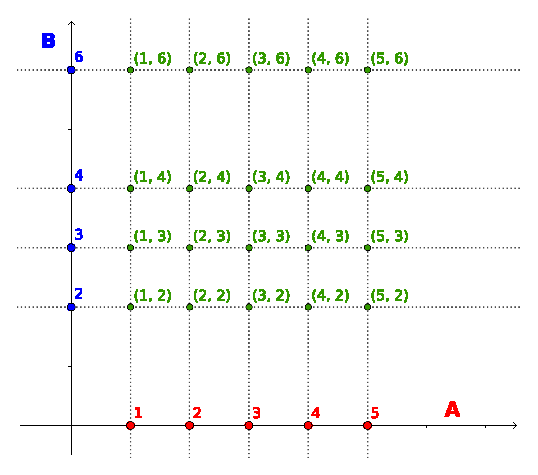
\includegraphics[width=7cm]{./cap_conjuntos/figs/ProdCartConj}}
    \caption{Produto cartesiano dos conjuntos $A$ e $B$}
  \end{figure}

 \end{exem}

\section{Cardinalidade de conjuntos}

 A \textbf{cardinalidade}\index{Conjunto(s)!cardinalidade de}\index{Conjunto(s)!número de elementos de} de um conjunto $A$ qualquer, é o número de elementos deste conjunto. Denotada por: $n(A)$, $|A|$ ou $\# A$.

 Note que: $n(\emptyset)= \# \emptyset= 0$.

 Dados dois conjuntos $A$ e $B$ quaisquer é importante observar que:
 \vskip0.3cm
 \colorbox{azul}{
 \begin{minipage}{0.9\linewidth}
 \begin{center}
 A cardinalidade da união destes dois conjuntos é dada por:
\begin{equation}
\#(A \cup B)= \# A + \# B - \#(A \cap B) .
\end{equation}
 \end{center}
 \end{minipage}}
 \vskip0.3cm

 Esta fórmula irá nos ajudar a resolver muitos problemas de teoria de conjuntos.

 \section{Conjunto das partes}

 Dado um conjunto $A$ o conjunto das partes de $A$ denotado por $\mathcal{P}(A)$ é o conjunto de todos os subconjuntos de $A$, ou seja,
\begin{equation}
\mathcal{P}(A)= \{X \mid X \text{ é um subconjunto de } A\} \ .
\end{equation}

 Dado um conjunto $A$ qualquer, precisamos ficar atentos a duas coisas:
 \begin{itemize}
 \item O conjunto $\emptyset$ sempre está no conjunto das partes de $A$, pois $\emptyset \subset A$;
 \item O conjunto $A$ sempre está no conjunto das partes de $A$, pois $A \subset A$.
 \end{itemize}
 Portanto, $\emptyset \in \mathcal{P}(A)$ e $A \in \mathcal{P}(A)$.

 \begin{exem}
 Se considerarmos o conjunto $A= \{a, b, c\}$, teremos pela definição acima que o conjuntos das partes de $A$ é:
\begin{equation}
\mathcal{P}(A)= \{ \emptyset, \{a\}, \{b\}, \{c\}, \{a, b\}, \{a, c\}, \{b, c\}, \{a, b, c\} \} \ .
\end{equation}
 \end{exem}

 E como sabemos se este conjunto acima contém de fato todos os subconjuntos do conjunto $A$? Bom para conseguirmos verificar isso vamos precisar utilizar a seguinte propriedade do conjunto das partes.

 \begin{prop}
  Se o conjunto $A$ possui $n$ elementos, então $\mathcal{P}(A)$ possui $2^n$ elementos. Ou seja:
\begin{equation}
\# A= n \ \ \Rightarrow \ \ \# \mathcal{P}(A)= 2^n \ .
\end{equation}
\end{prop}

 \begin{dem}
 Nesta demonstração utilizaremos o princípio fundamental da contagem\index{Princípio fundamental da contagem} para contar quantos subconjuntos um conjunto $A$ com $n$ elementos possui.

 Para começar considere um subconjunto $B$ qualquer de $A$. Observe que para cada um dos $n$ elementos de $A$, só existem duas possibilidades:
 \begin{itemize}
 \item Ou o elemento pertence ao subconjunto $B$;
 \item Ou o elemento não pertence ao subconjunto $B$.
 \end{itemize}

 Logo, pelo príncipio fundamental da contagem, nós podemos montar o conjunto $B$ de
\begin{equation}
\underbrace{2 \cdot 2 \cdot 2 \cdots 2}_{n-vezes}= 2^n
\end{equation}
 maneiras diferentes.

 E portanto, há $2^n$ subconjuntos de $A$ em $\mathcal{P}(A)$.
 \end{dem}

 Em nosso exemplo anterior temos que $\# A= 3$, logo aplicando esta propriedade obtemos que $\# \mathcal{P}(A)= 2^3= 8$, que é exatamente a quantidade de elementos que listamos no conjunto $\mathcal{P}(A)$, podemos com isso concluir que estes são todos os subconjuntos do conjunto $A$ que existem, portanto o conjunto $\mathcal{P}(A)$ está completo.



 \newpage
 \section{Propriedades das operações entre conjuntos}
 \index{Conjunto(s)!propriedades das operações entre}
 \index{Propriedades!das operações entre conjuntos}

 Dada uma família $\mathcal{A}$ de conjuntos, ou seja, dado um conjunto $\mathcal{A}$ de conjuntos, temos:
 \begin{itemize}
 \item União de todos os conjuntos que são elementos de $\mathcal{A}$:
\begin{equation}
\bigcup_{A \in \mathcal{A}} A = \{x\mid x \in A \text{ para algum } A \in \mathcal{A}\}
\end{equation}
 \item Interseção de todos os conjuntos que são elementos de $\mathcal{A}$:
\begin{equation}
\bigcap_{A \in \mathcal{A}} A = \{x\mid x \in A \text{ para todo } A \in \mathcal{A}\}
\end{equation}
\end{itemize}

\begin{prop}
Sejam $A$, $B$ e $C$ conjunto arbitrários, temos que:
\begin{itemize}
 \item $\emptyset \subset A$, $\forall A$
 \item $A \cup \emptyset= A$ e $A \cap \emptyset= \emptyset$
 \item $A \cap (B \cup C) = (A \cap B) \cup (A \cap C)$
 \item $A \cup (B \cap C) = (A \cup C) \cap (A \cup C)$
 \item $A - (B \cup C) = (A - B) \cap (A - C)$ (lei de DeMorgan)
 \item $A - (B \cap C) = (A - B) \cup (A - C)$ (lei de DeMorgan)
 \item $\bigcap_{\alpha \in J}(U_{\alpha} \cap Y) = (\bigcap_{\alpha \in J} U_{\alpha}) \cap Y$

\begin{equation}
(U_1 \cap Y) \cap \cdots \cap (U_n \cap Y) = (U_1 \cap \cdots \cap U_n) \cap Y
\end{equation}

 \item $\bigcup_{\alpha \in J}(U_{\alpha} \cap Y) = (\bigcup_{\alpha \in J} U_{\alpha}) \cap Y$

\begin{equation}
(U_1 \cap Y) \cup \cdots \cup (U_n \cap Y) = (U_1 \cup \cdots \cup U_n) \cap Y
\end{equation}

 \item $(U \times V) \cap (A \times B) = (U \cap A) \times (V \cap B)$

 \item $X - \bigcap_{\alpha \in J} A_{\alpha} = \bigcup_{\alpha \in J}(X - A_{\alpha})$

 \item $X - \bigcup_{i= 1}^{n} A_i = \bigcap_{i = 1}^{n}(X - A_i)$

\end{itemize}
\end{prop}

\section{Exercícios}

\construirExer

\begin{exer}
O coordenador de esportes de um clube, fez uma reunião com $22$ atletas que representam o clube nas modalidades de Handebol e Basquete, para repassar algumas instruções sobre o campeonato no qual o clube estava inscrito. Ele aproveitou para distribuir os novos uniformes conforme a equipe na qual o atleta participa, foram entregues $14$ uniformes de Handebol e $12$ uniformes de Basquete. Quantos atletas fazem parte apenas da equipe de Handebol?
\end{exer}
\begin{resp}
  $10$ atletas participam apenas da equipe de Handebol.
\end{resp}